\subsection{Design of the Graphical User Interface}
\label{subsec:designgui}

To come up with a proper design for the graphical user interface (GUI) of the application, it was decided to do a few brainstorming sessions, followed by sketching in an incremental approach. The goal for this approach was to quickly get an idea of what different elements could look like, and at the same time find out what could work and what would not. This is not to confuse with prototyping, as sketches are suggestive and quickly drawn, rather than prototypes that are attempts to mimic a final product.
The result of brainstorming and refining/discarding sketches was a common understanding of different ideas, providing a way to unite and improve them. Examples of such sketches can be seen in \ref{fig:prototype_brainstorming}. The sketches on the top row are early sketches of \texttt{LoginActivity} (left) and \texttt{SignUpActivity} (right). The bottom left sketch was an idea for recipe- and ingredient searching, while the bottom right was the first step towards the sliding screens used in the actual implementation - this eventually made it to become the \texttt{PagerActivity}.

\begin{figure}[H]
	\centering
	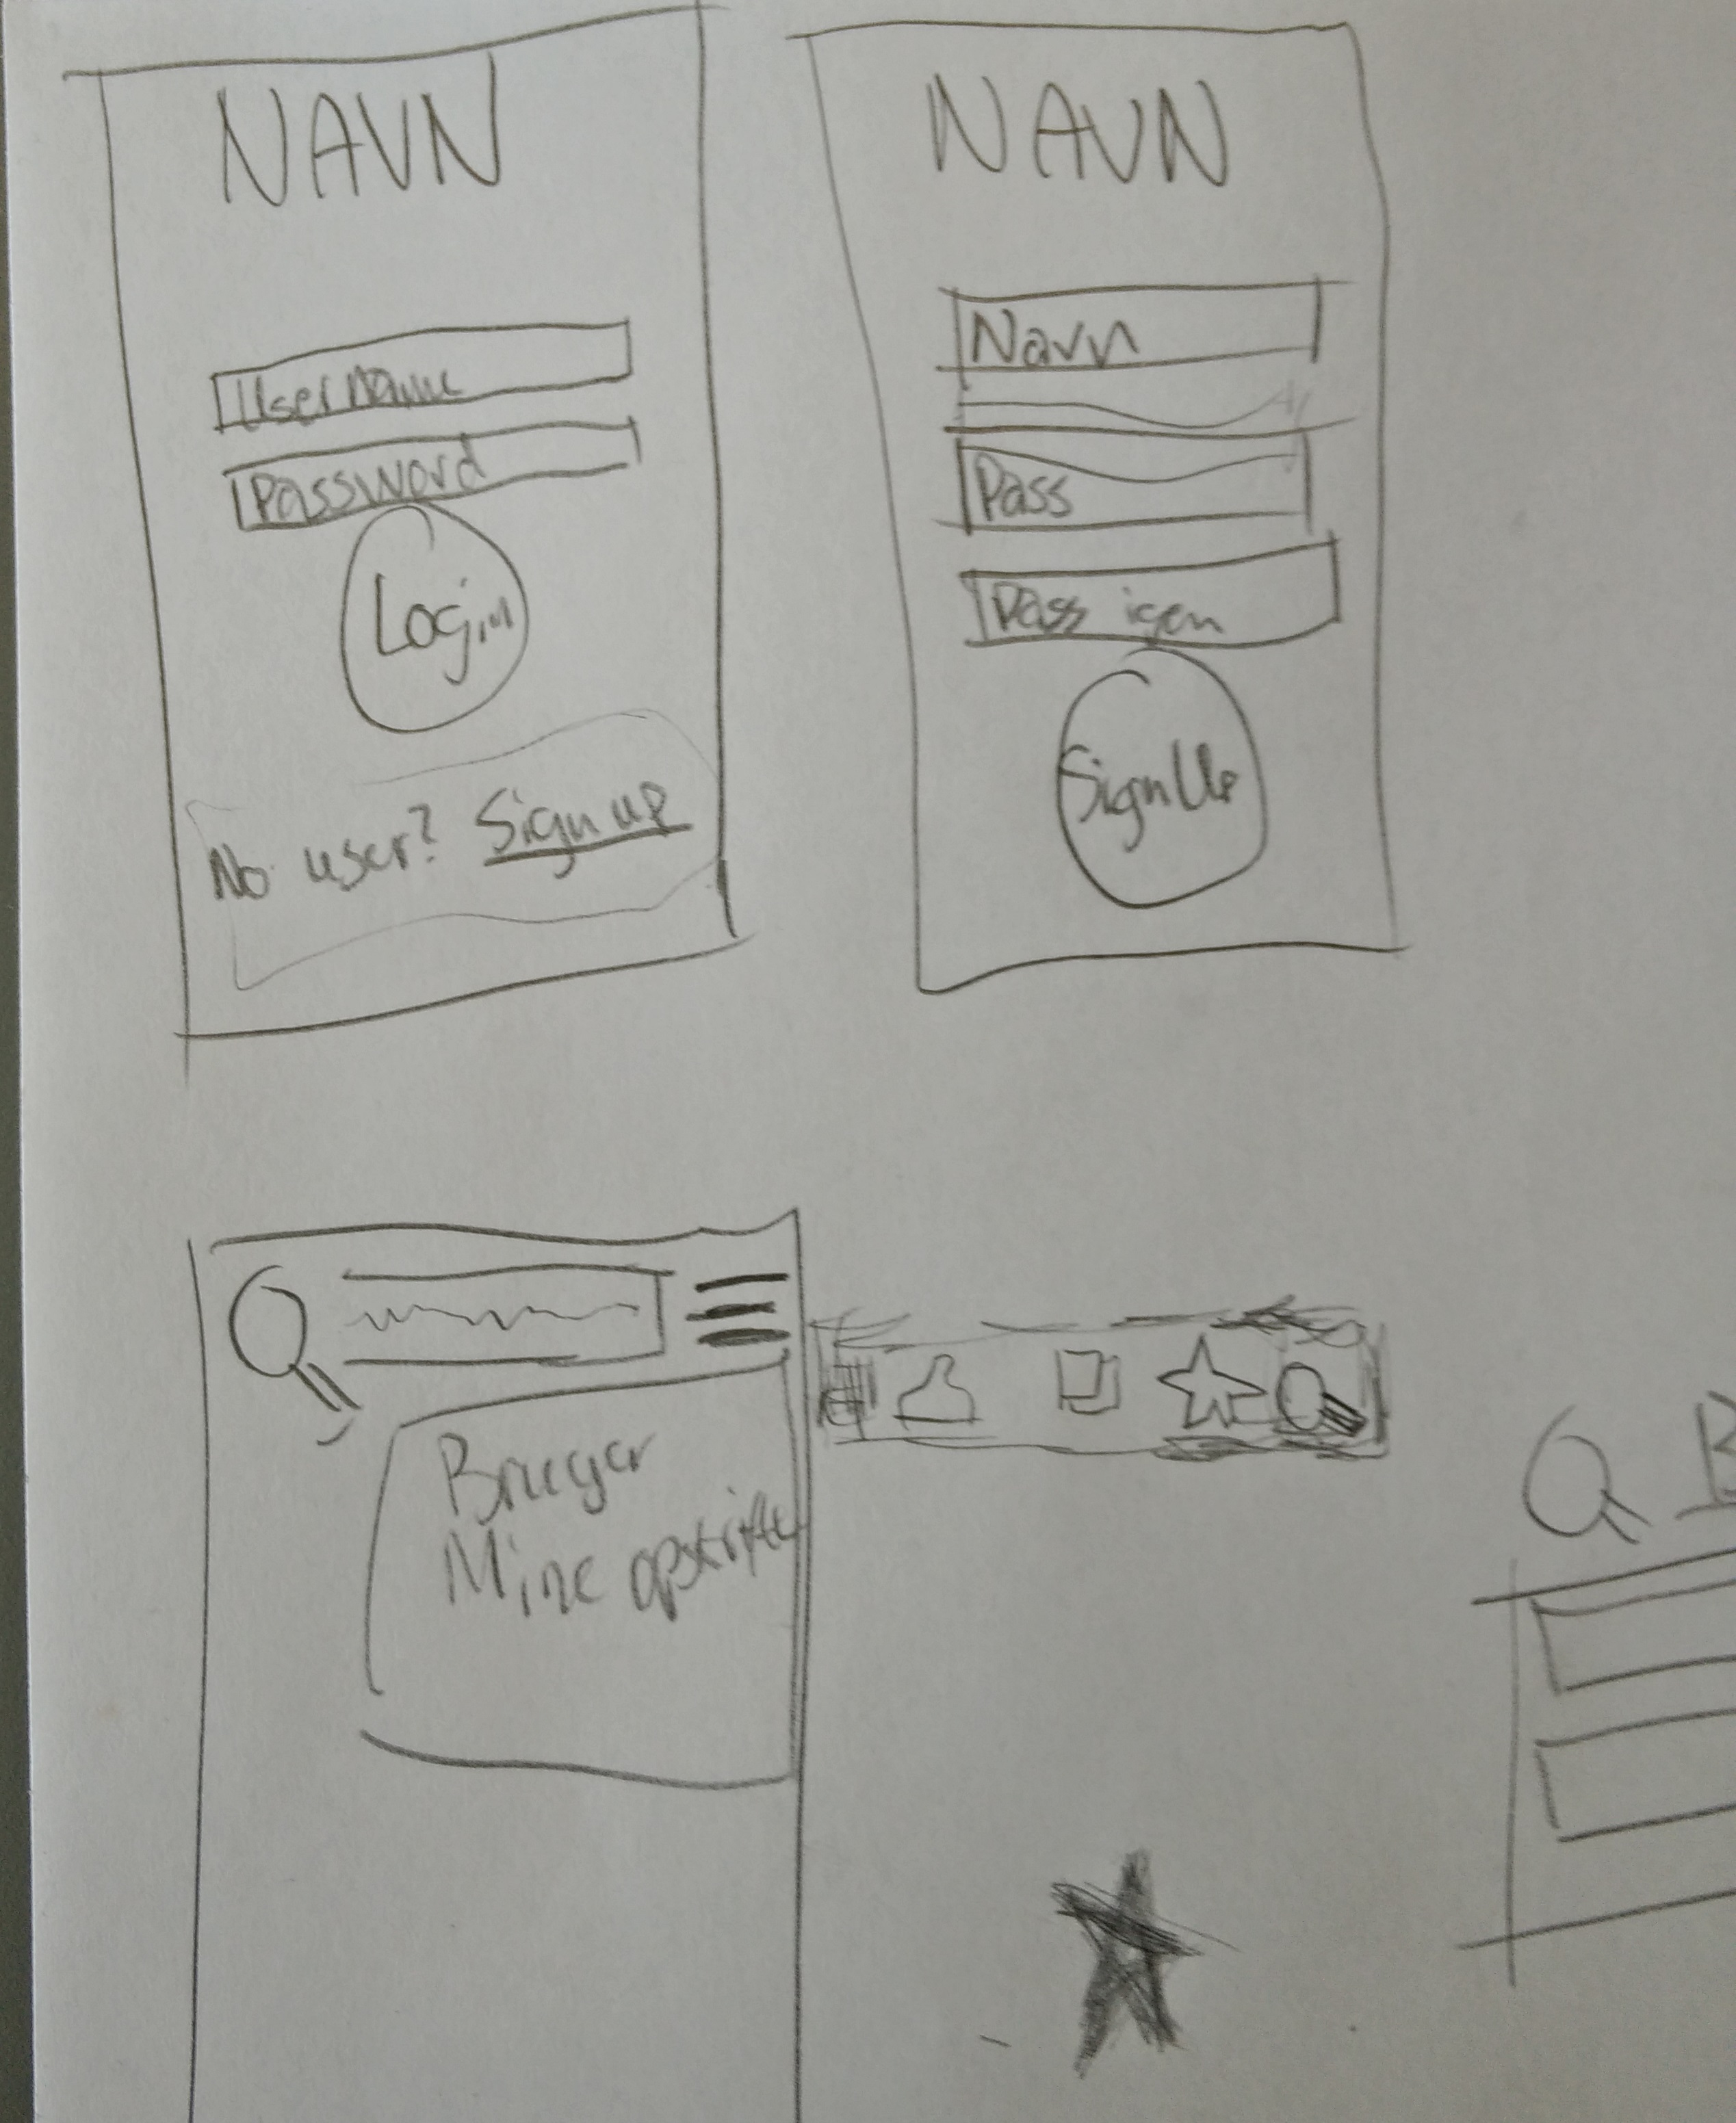
\includegraphics[width=\textwidth]{Pictures/prototype_brainstorming.jpg}
	\caption{Sketches of four different screens}
	\label{fig:prototype_brainstorming}
\end{figure}

After gathering the sketches into one united idea, prototyping was used to illustrate the product and provide a more definitive idea of how it would all come together. It should however be noted that since prototypes was done with just pen and paper, it was still acceptable to discard ideas that did not turn out as expected. The goal was to reach a more final design. Refinements of sketches can be seen in \ref{fig:prototype_login} and \ref{fig:prototype_pageractivity}. The former was rather simple, and did not change much compared to the sketches. The idea of sliding screens was greatly refined into the latter, a big change from the initial sketch. Finally the searching screen was discarded in favor of the "Discover" screen (second from the right).

The prototypes were used as basis for the application that was developed, and while a few alterations was made during development, the prototypes are still recognizable.

In spite of using both sketching and prototyping, the design phase was inexpensive in terms of time used. This was in great deal due to keeping both parts low fidelity.

\begin{figure}[H]
	\centering
	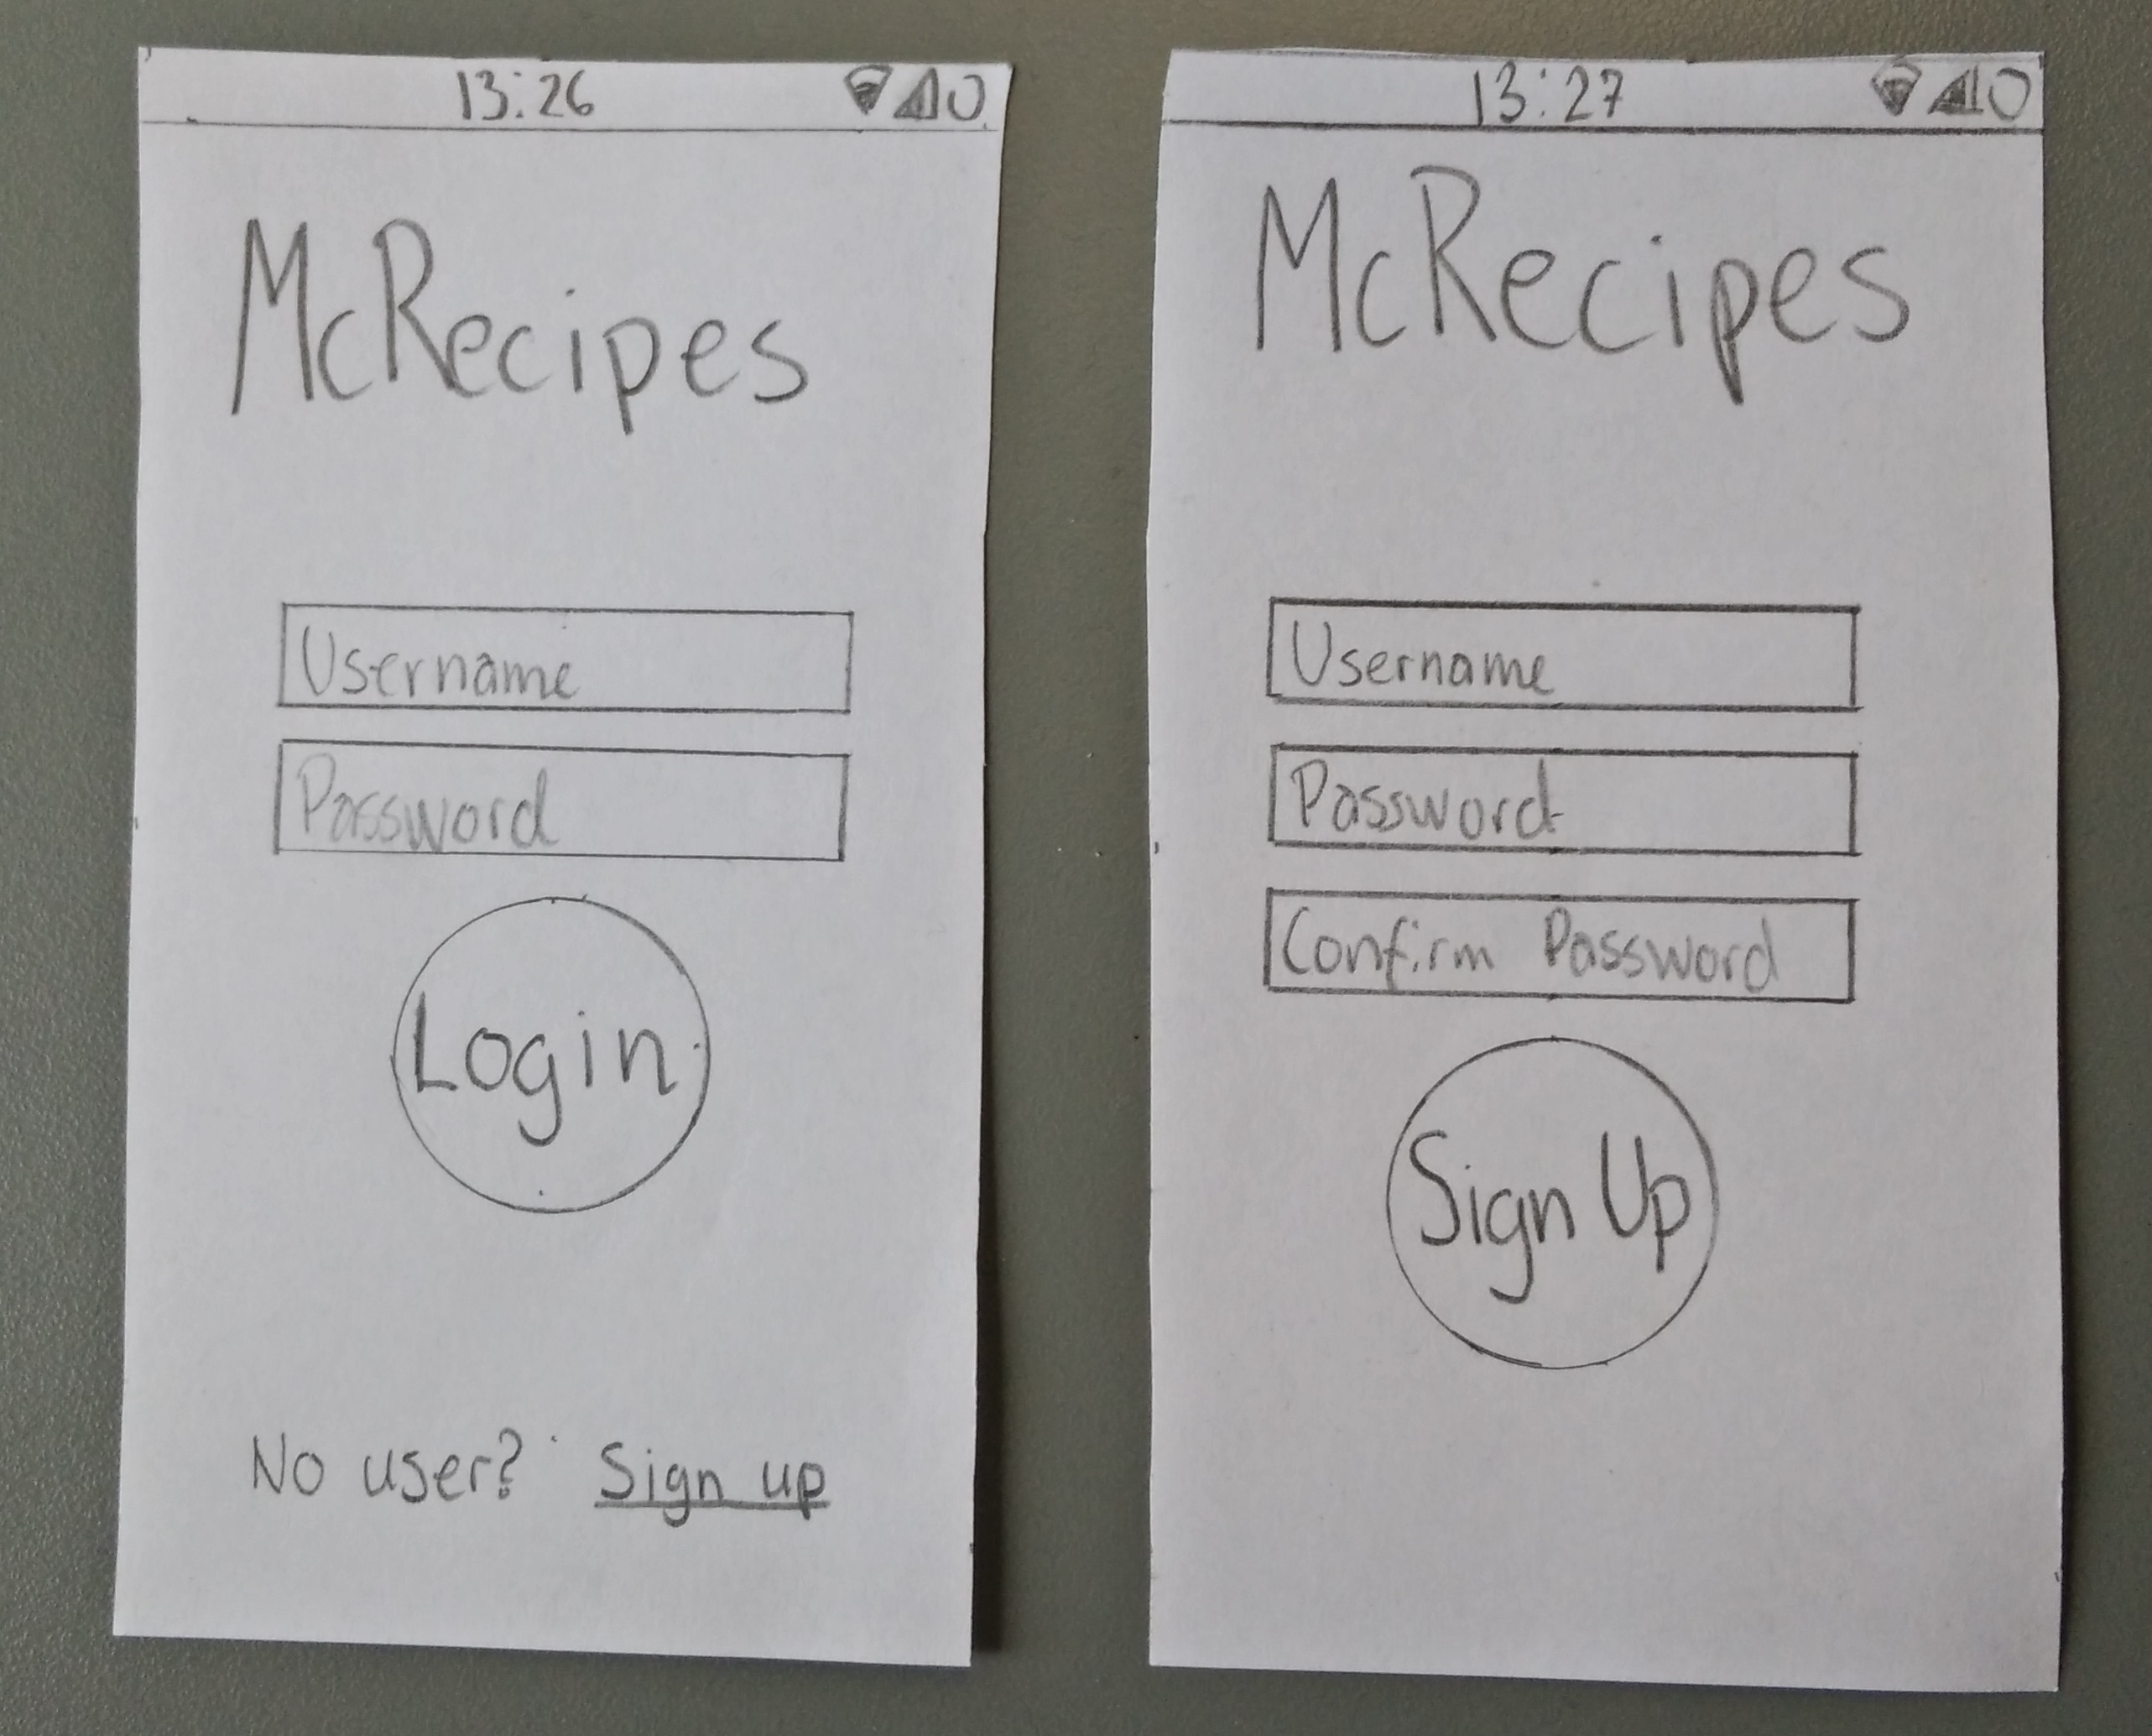
\includegraphics[width=\textwidth]{Pictures/prototype_login.jpg}
	\caption{The Login- and SignUpActivity as prototypes}
	\label{fig:prototype_login}
\end{figure}

\begin{figure}[H]
	\centering
	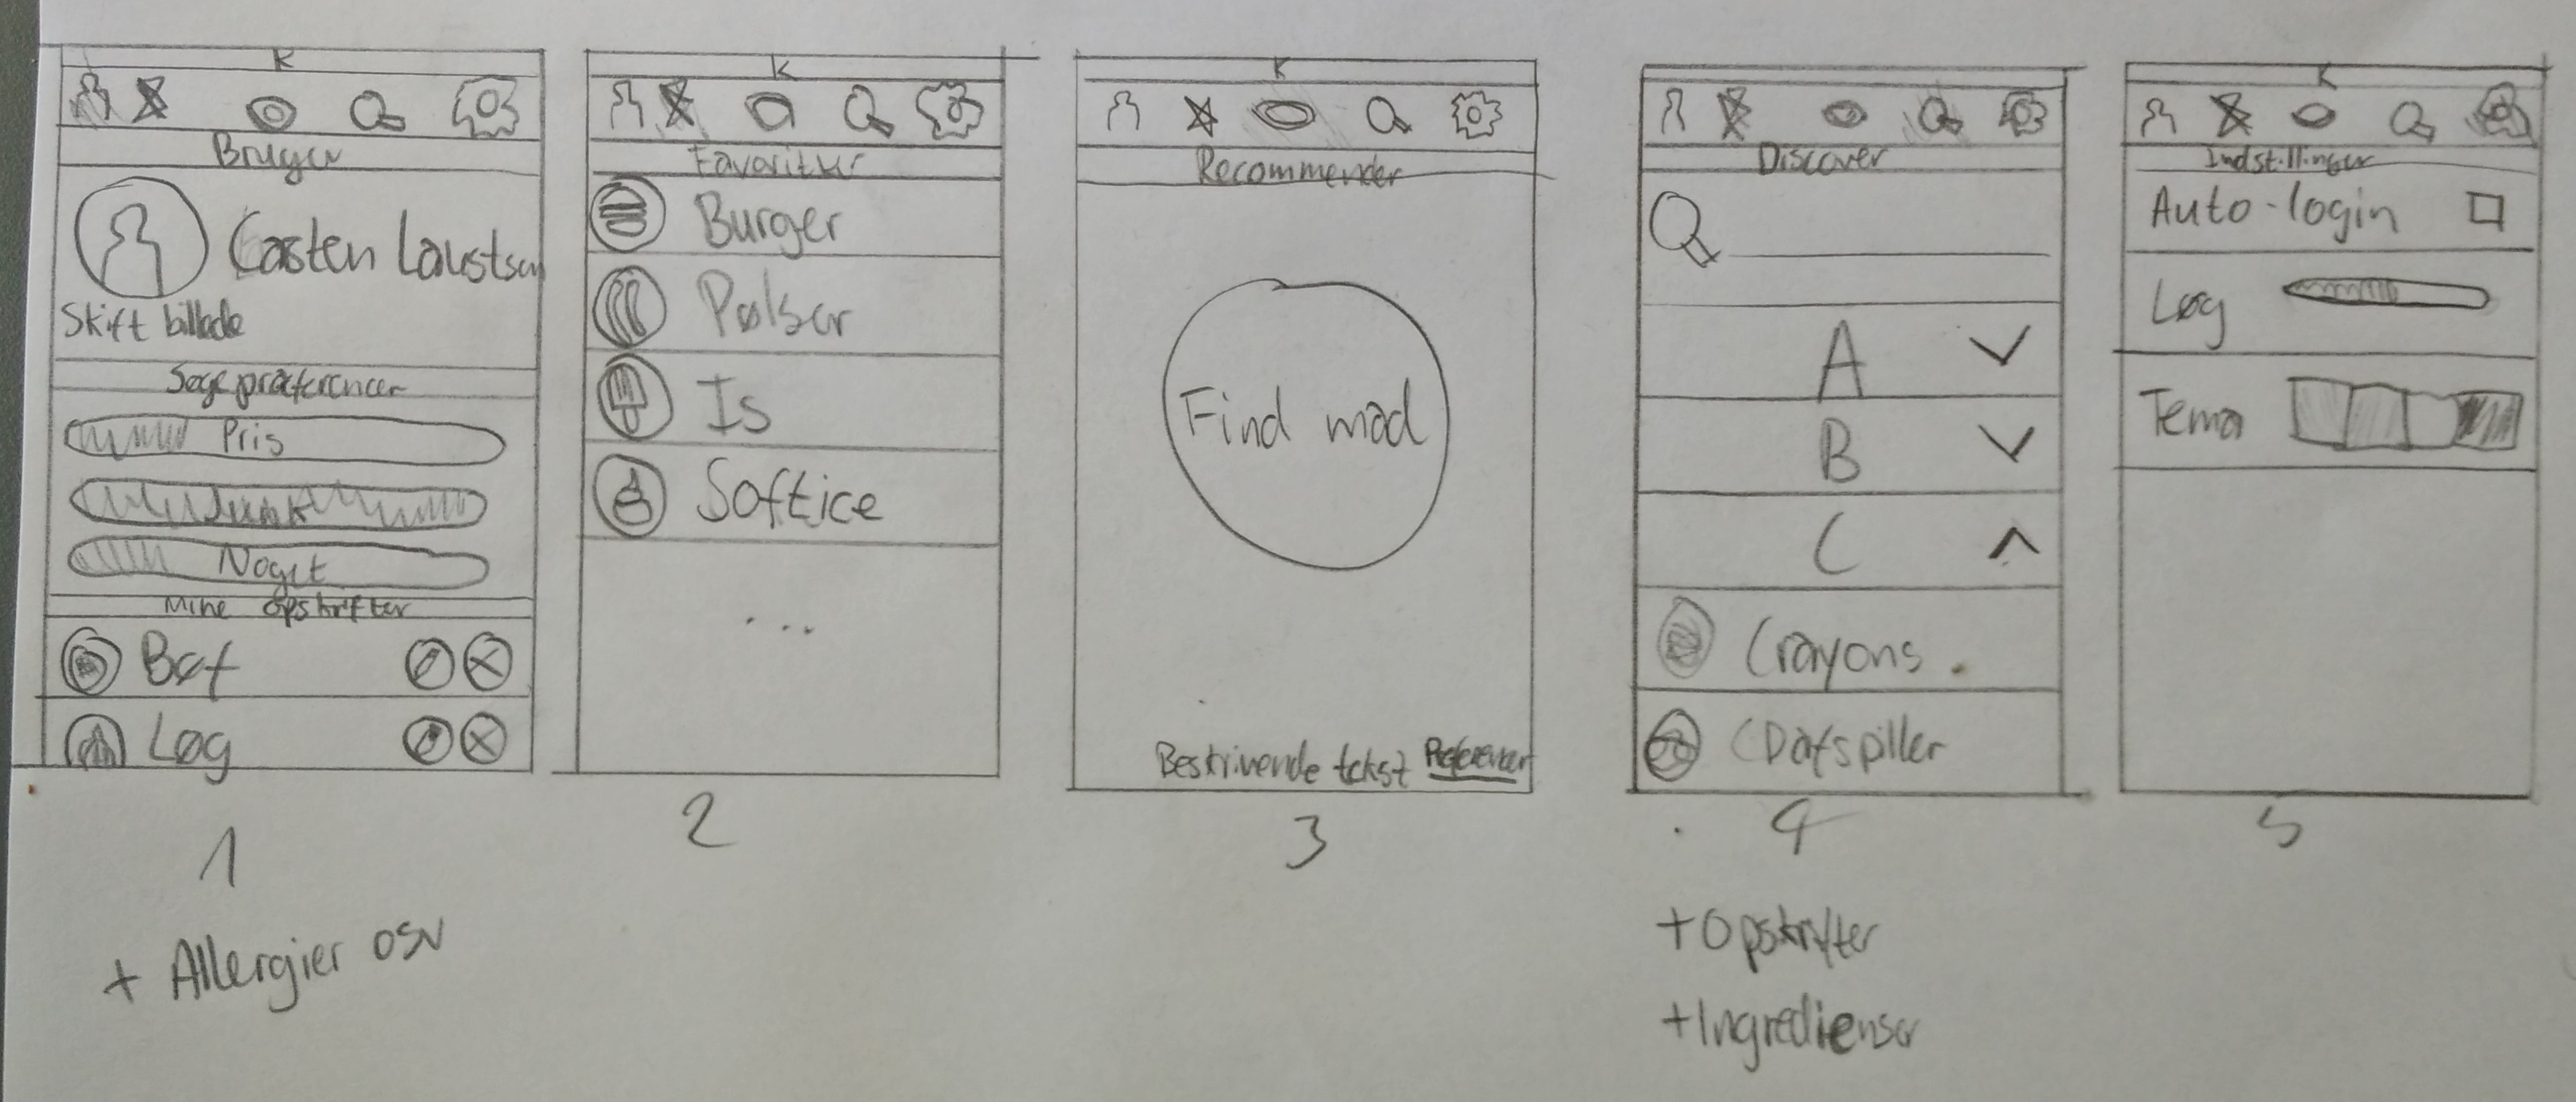
\includegraphics[width=\textwidth]{Pictures/prototype_pageractivity.jpg}
	\caption{Prototyping the PagerActivity}
	\label{fig:prototype_pageractivity}
\end{figure}

In addition to sketches and prototypes, it was also decided to focus on navigation in the early design phase. The application should be user friendly, which involved intuitive navigation through the program. As such, not only the GUI was modeled, but also navigation paths as can be seen in \ref{fig:prototype_structure}. The structure shown was discarded due to the introduction of paged screens, which was deemed a better idea for navigation. The chart ultimately turned into the figure, \ref{fig:application_navigation}. The navigation sketches helped ensure that functions would not be stuffed away somewhere that it did not make sense and provided a better overview of the solution that was built towards.

\begin{figure}[H]
	\centering
	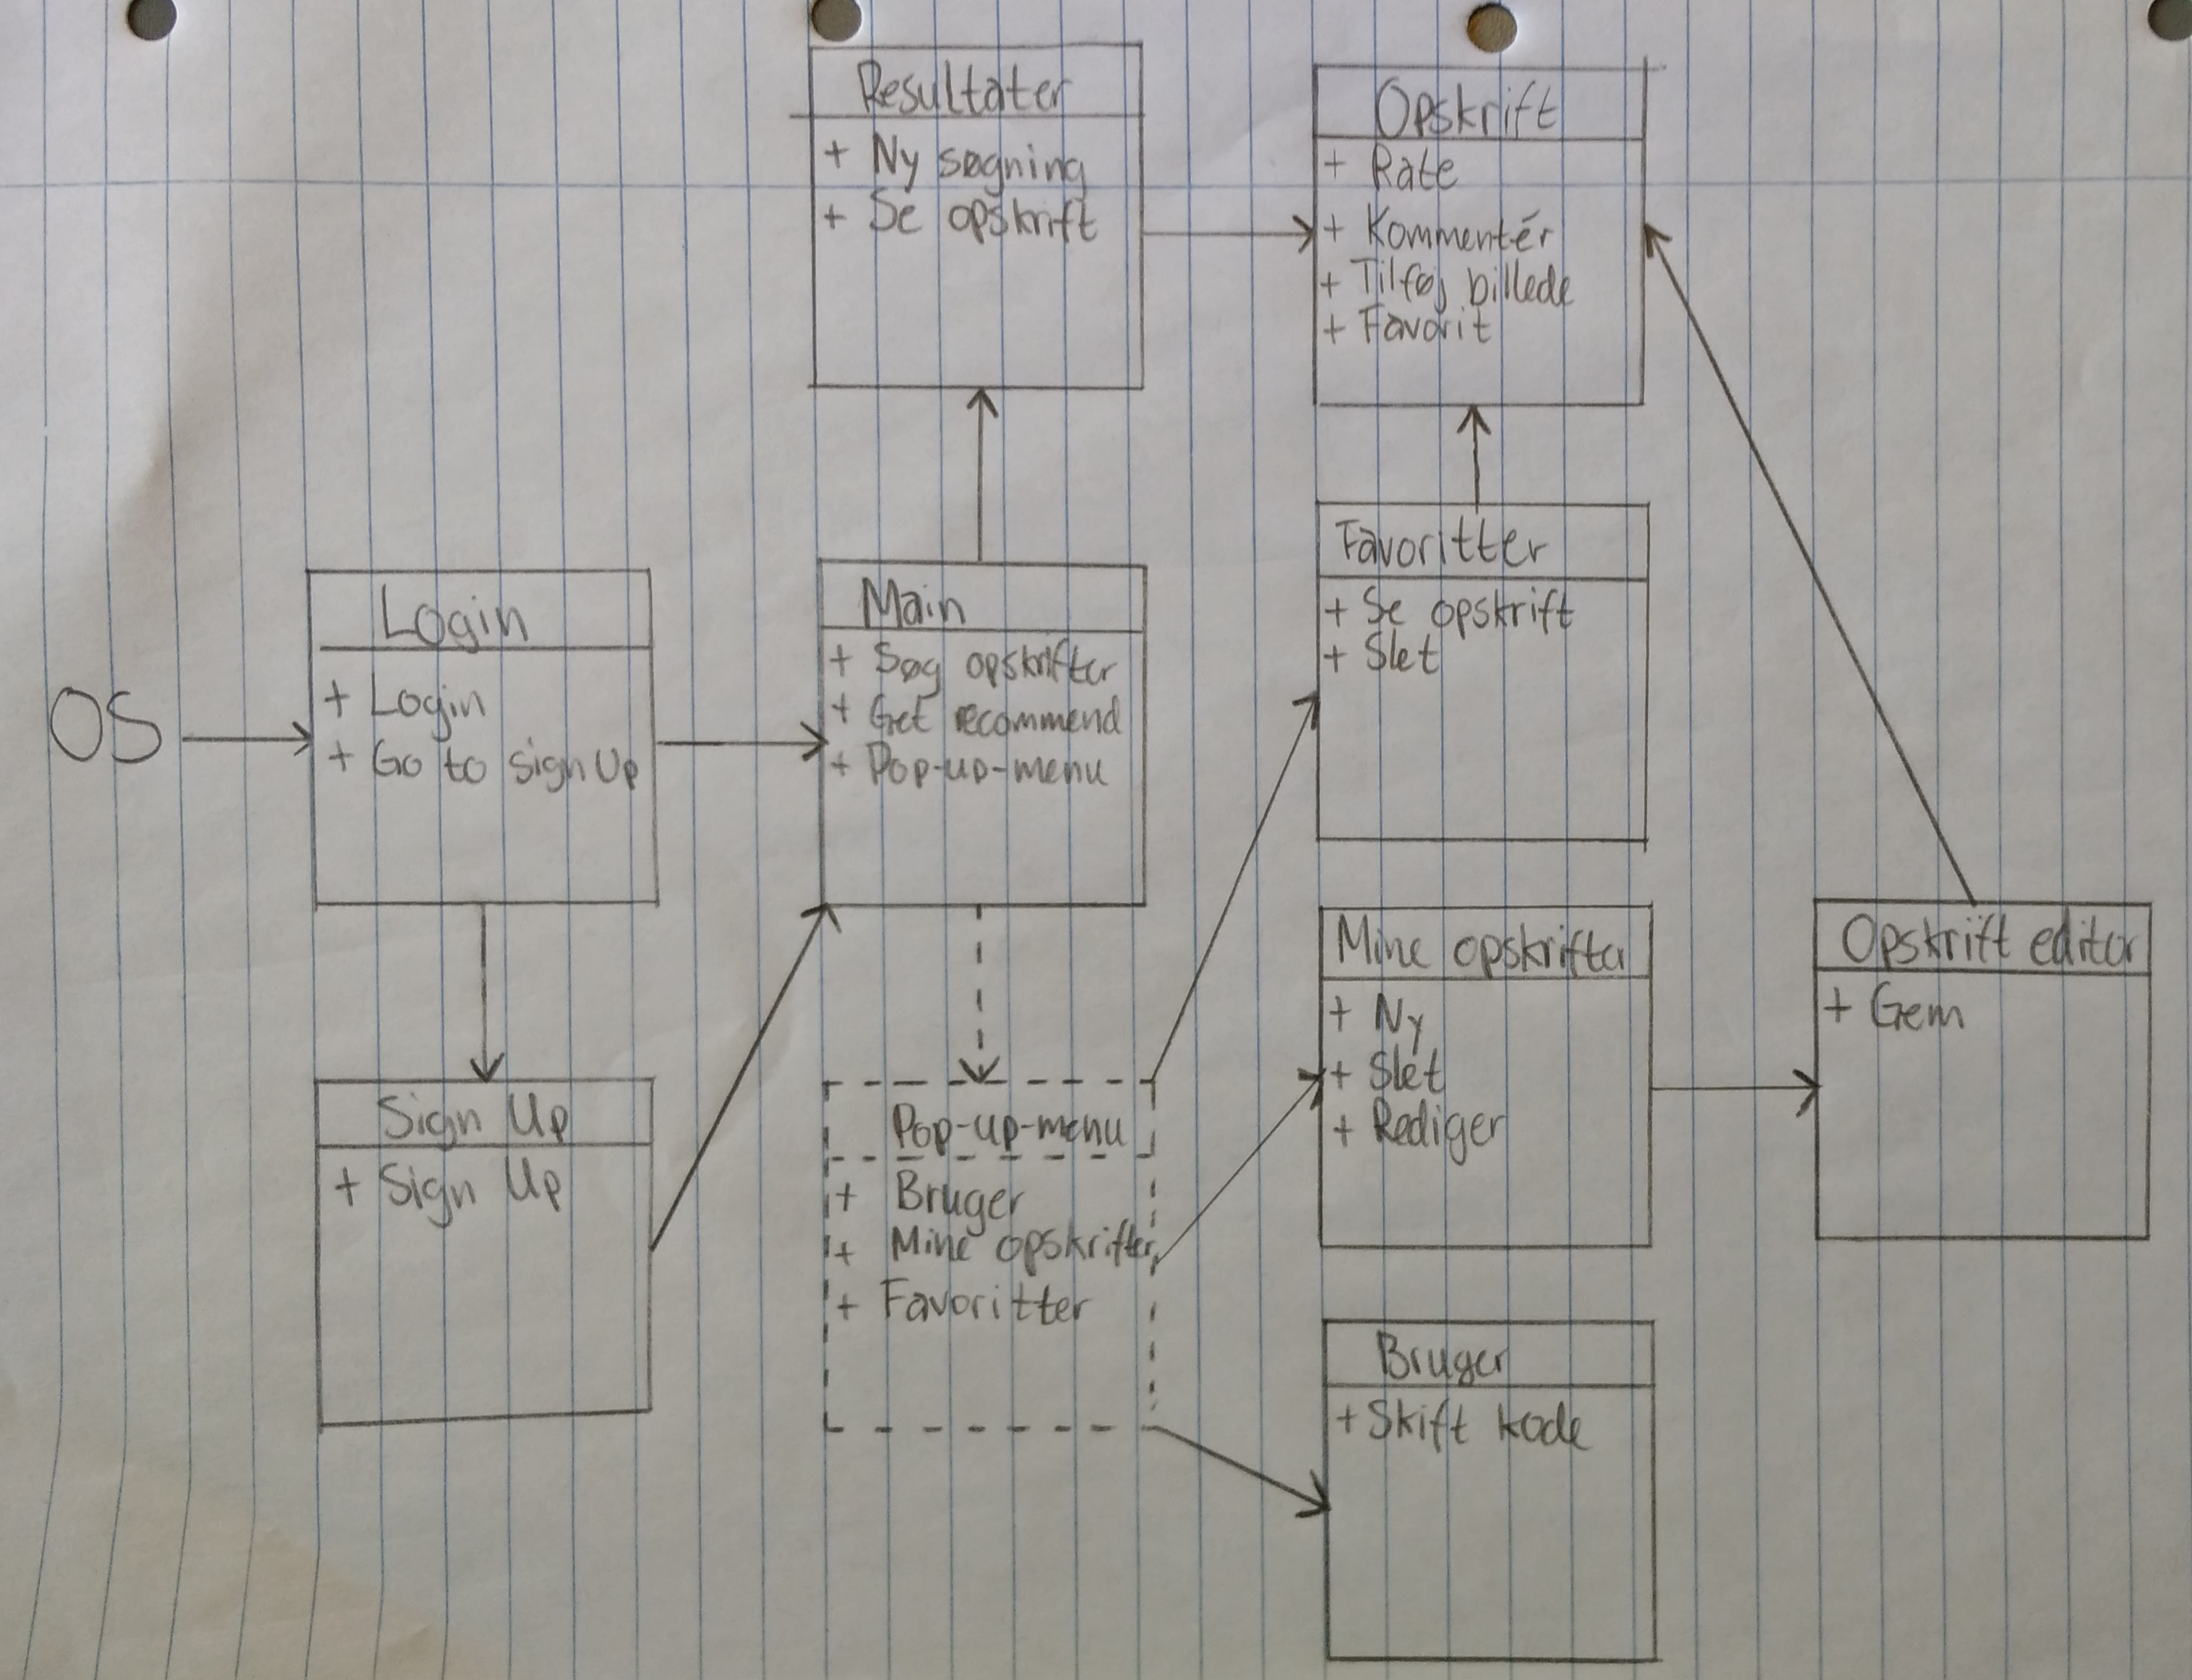
\includegraphics[width=\textwidth]{Pictures/prototype_structure.jpg}
	\caption{A discarded sketch of navigational structure}
	\label{fig:prototype_structure}
\end{figure}